%%
%% Copyright (c) 2018-2019 Weitian LI <liweitianux@sjtu.edu.cn>
%% Creative Commons BY 4.0
%%

\chapter{补充公式}
\label{app:formulas}


在本文所采用的平直 \lcdm 宇宙中,\acl{Ez} \acs{Ez} 为 \cite{hogg1999}:
\begin{align}
  \label{eq:Ez}
  \acs{Ez}
    & = \sqrt{\acs{Om0} (1+z)^3 + \Omega_k (1+z)^2 + \acs{Ol0}}  \\
    & = \sqrt{\acs{Om0} (1+z)^3 + \acs{Ol0}} \, .
\end{align}
于是,\acl{Hz}可表示为:
\begin{equation}
  \label{eq:hubble-z}
  \acs{Hz} = \acs{H0} \, \acs{Ez} .
\end{equation}
该红移处的宇宙临界密度为:
\begin{equation}
  \label{eq:rho-crit}
  \acs{rho-crit}(z) = \frac{3 H^2(z)}{8 \Cpi \acs{G}} ,
\end{equation}
其中 \acs{G} 是\acl{G}。


%=====================================================================
\section{维里半径和维里质量}

位于红移 $z$ 处的星系团的\acf{r-vir}定义为该半径范围内星系团的平均密度
是当时宇宙临界密度的 \acs{overdensity-vir} 倍,
由下式给出:
\begin{equation}
  \label{eq:radius-virial}
  \acs{r-vir}(z) = \left[
    \frac{3 \acs{M-vir}}{4\Cpi \acs{overdensity-vir} \acs{rho-crit}(z)}
  \right]^{1/3},
\end{equation}
其中 \acs{M-vir} 是星系团的\acl{M-vir}(通常用作其总引力质量),
\acf{overdensity} \acs{overdensity-vir} 为 \cite{bryan1998}:
\begin{equation}
  \label{eq:delta-vir}
  \acs{overdensity-vir}(z)
    = 18\Cpi^2 + 82 [\Omega_f(z) - 1] - 39 [\Omega_f(z) - 1]^2 ,
\end{equation}
其中 $\Omega_f(z)$ 是红移为 $z$ 时的宇宙物质密度参数:
\begin{equation}
  \label{eq:omega-f}
  \Omega_f(z) = \frac{(1+z)^3}{E^2(z)} \acs{Om0} .
\end{equation}


%=====================================================================
\section{%
  \texorpdfstring{$r_{200}$}{r200} 与 \texorpdfstring{$r_{500}$}{r500} 以及
  \texorpdfstring{$M_{200}$}{M200} 与 \texorpdfstring{$M_{500}$}{M500} 的换算}
\label{sec:r-m-conv}

实际情况中会经常用到星系团的 $r_{200}$ 和 $r_{500}$,分别定义为该半径范围内
星系团的平均密度是当时宇宙临界密度的 200 和 500 倍。
于是,$M_{200}$ 和 $M_{500}$ 分别为 $r_{200}$ 和 $r_{500}$ 之内的总质量。
一般可认为 $r_{200} \simeq \acs{r-vir}$
以及 $r_{500} \simeq 0.65 \, r_{200}$ \cite{ettori2009},
因此 $M_{200} \simeq \acs{M-vir}$,
而 $M_{200}$ 和 $M_{500}$ 之间的换算可参考下述方法。

假定星系团的密度分布符合 \ac{nfw} 模型\cite{navarro1997}:
\begin{equation}
  \label{eq:nfw}
  \rho(r) = \frac{\rho_s}{
    (r / r_s) (1 + r / r_s)^2} \,,
\end{equation}
其中 $\rho_s$ 是密度参数,$r_s$ 是标度半径 (scale radius)。
于是半径 $r = s \,\acs{r-vir}$ 之内的总质量可表示为\cite{lokas2001}:
\begin{equation}
  \label{eq:mass-r}
  M(< s \,\acs{r-vir}) = \acs{M-vir}
    \frac{\ln(1 + c s) - c s / (1 + c s)}{\ln(1 + c) - c / (1 + c)} ,
\end{equation}
其中 $c = \acs{r-vir} / r_s$ 为聚集参数 (concentration parameter)。
\citeay{duffy2008} 通过数值模拟研究得出该参数与质量存在如下关系:
\begin{equation}
  \label{eq:mass-c}
  c = A \left( \frac{M_{200}}{M_{\R{pivot}}} \right)^B (1+z)^C ,
\end{equation}
其中 $M_{\R{pivot}} = \SI{2e12}{\per\hubble\solarmass}$,
$A = 5.71$, $B = -0.084$, 以及 $C = 0.47$。
利用上述两式便可由 $M_{200}$ 换算得到 $M_{500}$;
反过来并利用迭代法,亦可由 $M_{500}$ 导出 $M_{200}$。


%=====================================================================
\section{暗物质塌缩的临界密度}

在 \ac{cdm} 模型中,暗物质塌缩形成暗物质晕的\acl{delta-crit}
(critical linear overdensity)
随红移的变化关系可表示为 \cite{kitayama1996,randall2002}:
\begin{equation}
  \label{eq:delta-crit}
  \acs{delta-crit} = \frac{D(z=0)}{D(z)}
    \frac{3 (12\Cpi)^{2/3}}{20}
    \left[1 + 0.0123 \log_{10} \Omega_f(z) \right] ,
\end{equation}
其中 $D(z)$ 是增长因子 (growth factor),可由下述公式计算
[参见 \citeay{peebles1980}, 式~(13.6)]:
\begin{equation}
  \label{eq:growth-factor}
  D(x) = \frac{(x^3 + 2)^{1/2}}{x^{3/2}}
    \mathlarger{\int_0^x} y^{3/2} (y^3 + 2)^{-3/2} \,\D{y} ,
\end{equation}
并且 $x_0 \equiv (2 \acs{Ol0} \big/ \acs{Om0})^{1/3}$,
$x = x_0 \big/ (1+z)$。


%=====================================================================
\section{宇宙年龄与红移的关系}

在平直宇宙学模型中,宇宙在红移 $z$ 时的年龄 $t$ 具有如下解析计算形式
[参见 \citeay{thomas2000}, 式~(18)]:
\begin{align}
  \label{eq:universe-age}
  t(z; \acs{Om0})
    & = \frac{1}{\acs{H0}} \mathlarger{\int_z^{\infty}}
      \!\frac{\D{z'}}{(1+z')\sqrt{1 + z' (3+3z'+z'^2) \acs{Om0}}}
      \nonumber \\
    & = \frac{2}{3 \acs{H0} \sqrt{\,1-\acs{Om0}}} \sinh^{-1}
      \!\left( \sqrt{\frac{\Omega_m^{-1} - 1}{(1+z)^3}} \right) .
\end{align}


%=====================================================================
\section{共动距离、光度距离和⻆直径距离}

两个相邻物体之间的\acl{D-comoving} (comoving distance)
$\delta\acs{D-comoving}$ 定义为,
当两者随 Hubble 流共同运动时,该距离 $\delta\acs{D-comoving}$ 保持不变
\cite{hogg1999}。
所以,$\delta\acs{D-comoving}$ 等于这两个物体之间的
固有距离 (proper distance) 乘以 $(1+z)$。
因此,一个位于红移 $z$ 的物体的(视向)\acl{D-comoving}
$\acs{D-comoving}(z)$ 为 \cite{hogg1999}:
\begin{equation}
  \label{eq:distance-comoving}
  \acs{D-comoving}(z)
    = \int_0^z \delta\acs{D-comoving}(z')\,\D{z'}
    = D_{\!H} \int_0^z \frac{\D{z'}}{E(z')} .
\end{equation}
其中 $D_{\!H} \equiv c / H_0$ 为 Hubble 距离。
在平直宇宙中,\acf{D-comoving-t} 与视向\acl{D-comoving}相等,即
\begin{equation}
  \label{eq:distance-comoving-t}
  \acs{D-comoving-t}(z) = \acs{D-comoving}(z) ,
    \quad \text{for } \Omega_k = 0 .
\end{equation}

一个物体的\acf{D-luminosity}由以下关系定义:
\begin{equation}
  \label{eq:dl-def}
  \acs{D-luminosity} \equiv
    \sqrt{\frac{L_{\R{bolo}}}{4\Cpi S_{\R{bolo}}}} ,
\end{equation}
其中 $L_{\R{bolo}}$ 是该物体的本征热光度 (bolometric luminosity),
$S_{\R{bolo}}$ 是测得的热流量 (bolometric flux)。
这里的 $L_{\R{bolo}}$ 和 $S_{\R{bolo}}$ 都是对全频段的积分值。

一个物体的\acf{D-angular}
定义为该物体的物理横向尺寸与其对观测者的张角(以 \si{radian} 为单位)之比。
需要注意的是,由于宇宙膨胀的原因,该距离并\emph{不}随红移单调递增,
即相同物理尺寸的物体位于更高红移(如 $z \gtrsim 1$)处时反而看起来更大
\cite{hogg1999}。
参见\autoref{fig:distance-measures},其中对比了三种宇宙距离测量随红移的变化。

\begin{figure}[htp]
  \centering
  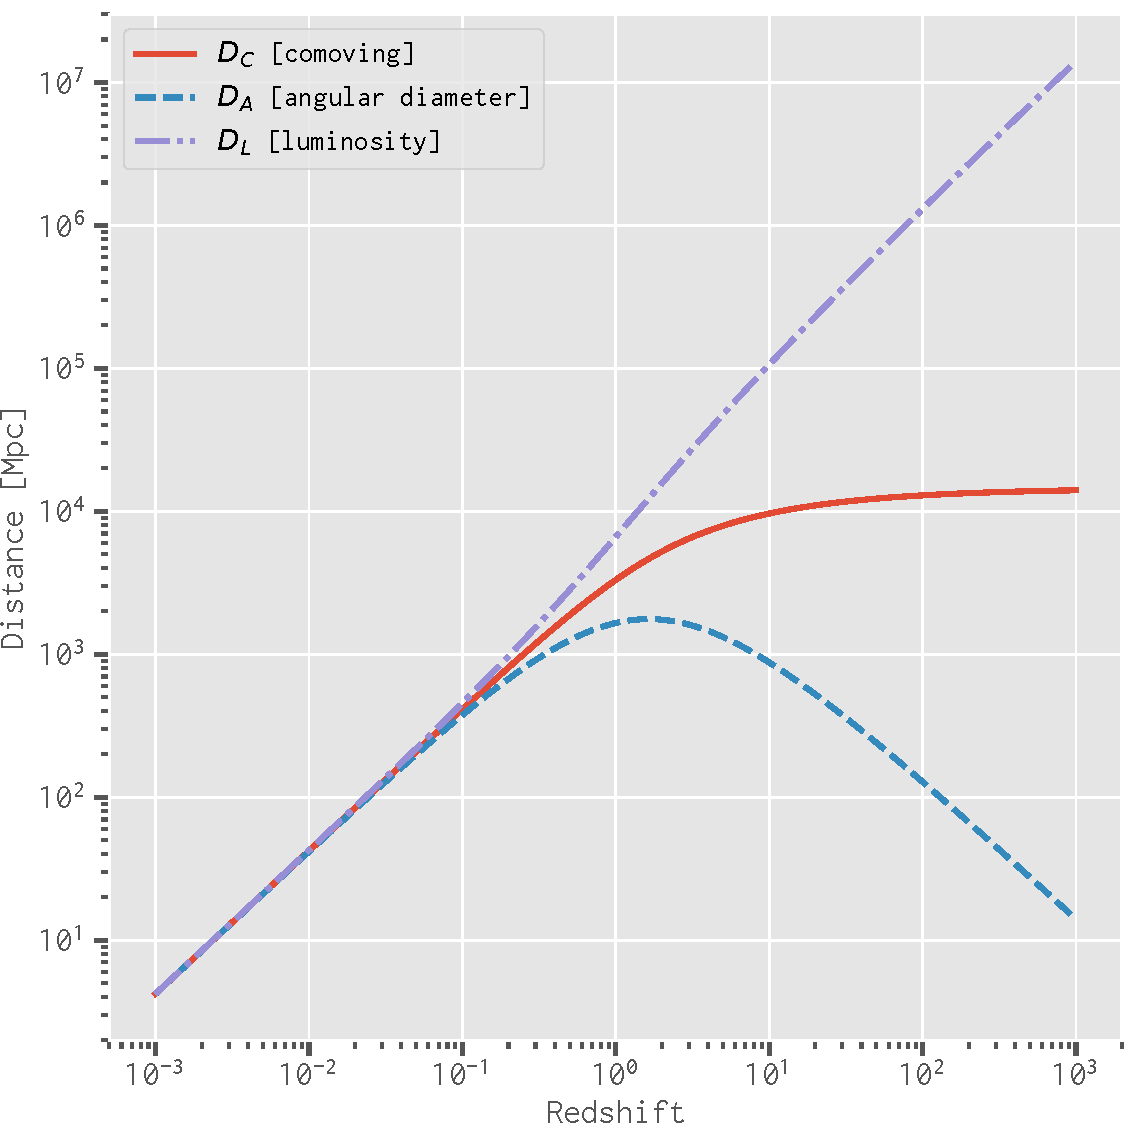
\includegraphics[width=0.8\textwidth]{distances-comparison}
  \bicaption[共动距离、光度距离和⻆直径距离随红移的变化]{%
    \acl*{D-comoving} $\acs*{D-comoving}(z)$、
    \acl*{D-angular} $\acs*{D-angular}(z)$
    和\acl*{D-luminosity} $\acs*{D-luminosity}(z)$
    三种宇宙距离测量从红移 $z = \num{e-3}$ 至 $z = \num{e3}$ 的变化情况。
  }{%
    A comparison among the comoving distance $\acs*{D-comoving}(z)$,
    angular diameter distance $\acs*{D-angular}(z)$, and
    luminosity distance $\acs*{D-luminosity}(z)$,
    from redshift $z = \num{e-3}$ to $z = \num{e3}$.
  }
  \label{fig:distance-measures}
\end{figure}

一个位于红移 $z$ 的物体,
其\acl{D-luminosity}与\acl{D-angular}之间有以下关系
\cite{weinberg1972,hogg1999,ellis2007}:
\begin{equation}
  \label{eq:dl-da}
  \acs{D-luminosity}(z) = (1+z)^2 \acs{D-angular}(z) .
\end{equation}


%=====================================================================
\section{波数与尺度的换算}
\label{sec:wavenumber-scale-conv}

Fourier 空间的\ac{wavenumber} \ac{k} 与实空间(即图像空间)的尺度 \ac{scale}
之间的换算关系为 \cite{peebles1980,baugh2000}:
\begin{equation}
  \ac{k} = 2\Cpi / \ac{scale} .
\end{equation}

EoR 信号的\ac{ps}研究中通常采用\ac{comoving-frame},
其中\ac{wavenumber} \ac{k} 的单位通常为 [\si{\per\Mpc}]。
然而在观测研究中,更习惯使用角分或角秒来描述尺度 \ac{scale}。
为了进行 \ac{k} 和 \ac{scale} 两者的换算,
首先需要计算 EoR 信号源(即中性氢云)的\acl{D-comoving}:
\begin{equation}
  \ac{D-comoving}(z) =
    \ac{D-comoving}(z = \ac{freq21cm} / \ac{freq} - 1) ,
\end{equation}
其中 \ac{freq} 是观测频率,\ac{freq21cm} 是\acl{freq21cm}。
于是可得换算关系为:
\begin{equation}
  \left( \frac{\ac{k}}{\si{\per\Mpc}} \right) =
    2\Cpi \left( \frac{\si{\Mpc}}{\ac{D-comoving}(z)} \right)
    \left( \frac{\si{rad}}{\ac{scale}} \right) ,
\end{equation}
相应的逆换算关系为:
\begin{equation}
  \left( \frac{\ac{scale}}{\si{rad}} \right) =
    2\Cpi \left( \frac{\si{\Mpc}}{\ac{D-comoving}(z)} \right)
    \left( \frac{\si{\per\Mpc}}{\ac{k}} \right) .
\end{equation}

以本文使用的三个频带的中心频率 124、158 和 196 MHz 为例,
\ac{wavenumber} \ac{k} 和空间尺度 \ac{scale} 的换算关系
如\autoref{tab:k-s-conv} 所示:

\begin{table}[htp]
  \centering
  \bicaption{%
    波数与尺度在 124、158 和 196 MHz 的换算关系
  }{%
    The conversion relations between the wavenumber and scale
    at 124, 158 and 196 MHz.
  }
  \label{tab:k-s-conv}

  \begin{tabular}{cccc}
    \toprule
    物理量 & \SI{124}{\MHz} & \SI{158}{\MHz} & \SI{196}{\MHz} \\
    \midrule
    红移 $z$ & 10.45 & 7.99 & 6.25 \\
    共动距离 \ac*{D-comoving}(z) &
      \SI{9762.6}{\Mpc} & \SI{9144.9}{\Mpc} & \SI{8529.8}{\Mpc} \\
    \midrule
    波数 $\ac*{k} = \SI{1}{\per\Mpc}$ &
      \SI{2.21}{\arcminute} & \SI{2.36}{\arcminute} & \SI{2.53}{\arcminute} \\
    尺度 $\ac*{scale} = \SI{1}{\arcminute}$ &
      \SI{2.21}{\per\Mpc} & \SI{2.36}{\per\Mpc} & \SI{2.53}{\per\Mpc} \\
    \bottomrule
  \end{tabular}
\end{table}


%% EOF
